\lcTex{%
  \newlength{\widthExtra}\setlength{\widthExtra}{1.1cm}
  \newlength{\widthLineReal}\setlength{\widthLineReal}{\linewidth}
  \addtolength{\widthLineReal}{-\widthExtra}
  \newlength{\minipageSpace}\setlength{\minipageSpace}{0.2cm}

  \newlength{\widthLeft}
  \newlength{\widthRight}
}

\newcommand{\reals}{{\rm I\!\hspace{-0.025em} R}}
\newcommand{\calC}{{\cal C}}
\newcommand{\calA}{{\cal A}}
\newcommand{\eps}{{\varepsilon}}
\newcommand{\dcel}{{\sc Dcel}}
\newcommand{\naive}{na\"{\i}ve}
\newcommand{\kdtree}{{\sc Kd}-tree}

% ===============================================================
\section{Introduction}
\label{bobs_sec:intro}
% ===============================================================
%
\begin{figure}[!htp]
\begin{ccTexOnly}
\begin{center}
\begin{tabular}{cccc}
  \pspicture[](-1,-2.3)(1,2)
    \psset{unit=1cm,linewidth=1pt}
    \pscircle*[linecolor=gray](0,-1){1}
    \pscircle*[linecolor=gray](0,1){1}
    \pscircle(0,-1){1}
    \pscircle(0,1){1}
    \psline{->}(0,0)(0,1)
    \psline{->}(0,0)(1,0)
  \endpspicture &
  \pspicture[](-2,-2.3)(2,2)
    \psset{unit=1cm,linewidth=1pt}
    \pscircle*[linecolor=gray](-1,0){1}
    \pscircle*[linecolor=gray](1,0){1}
    \pscircle(-1,0){1}
    \pscircle(1,0){1}
    \psline{->}(0,0)(0,1)
    \psline{->}(0,0)(1,0)
  \endpspicture &
  \pspicture[](-2,-2.3)(2,2)
    \psset{unit=1cm,linewidth=1pt}
    \pscustom[linewidth=0,fillstyle=solid,fillcolor=gray]{
      \psarc(0,1){1}{270}{360}
      \psarc(1,0){1}{90}{180}
    }
    \pscustom[linewidth=0,fillstyle=solid,fillcolor=gray]{
      \psarc(1,0){1}{180}{270}
      \psarc(0,-1){1}{0}{90}
    }
    \pscustom[linewidth=0,fillstyle=solid,fillcolor=gray]{
      \psarc(0,-1){1}{90}{180}
      \psarc(-1,0){1}{270}{360}
    }
    \pscustom[linewidth=0,fillstyle=solid,fillcolor=gray]{
      \psarc(-1,0){1}{0}{90}
      \psarc(0,1){1}{180}{270}
    }
    \psarc(0,1){1}{270}{360}
    \psarc{c}(1,0){1}{90}{180}
    \psarc(1,0){1}{180}{270}
    \psarc{c}(0,-1){1}{0}{90}
    \psarc(0,-1){1}{90}{180}
    \psarc{c}(-1,0){1}{270}{360}
    \psarc{-c}(-1,0){1}{0}{90}
    \psarc(0,1){1}{180}{270}
  \endpspicture &
  \pspicture[](-2,-2.3)(2,2)
    \psset{unit=1cm,linewidth=1pt}
    \pscustom[linewidth=0,fillstyle=solid,fillcolor=gray,linecolor=gray]{
      \psarc(0,1){1}{360}{180}
      \psarc(1,0){1}{90}{180}
      \psarc(-1,0){1}{0}{90}
    }
    \pscustom[linewidth=0,fillstyle=solid,fillcolor=gray,linecolor=gray]{
      \psarc(1,0){1}{270}{90}
      \psarc(0,-1){1}{0}{90}
      \psarc(0,1){1}{270}{0}
    }
    \pscustom[linewidth=0,fillstyle=solid,fillcolor=gray,linecolor=gray]{
      \psarc(0,-1){1}{180}{0}
      \psarc(-1,0){1}{270}{360}
      \psarc(1,0){1}{180}{270}
    }
    \pscustom[linewidth=0,fillstyle=solid,fillcolor=gray,linecolor=gray]{
      \psarc(-1,0){1}{90}{270}
      \psarc(0,1){1}{180}{270}
      \psarc(0,-1){1}{90}{180}
    }
    \pscircle(0,-1){1}
    \pscircle(0,1){1}
    \pscircle(-1,0){1}
    \pscircle(1,0){1}
  \endpspicture\\
  & & intersection & symmetric difference
\end{tabular}
\end{center}

\end{ccTexOnly}
\begin{ccHtmlOnly}
  <p><center>
    <img src="./fig/teaser.gif" border=0 alt="Boolean Set Operations">
  </center>
\end{ccHtmlOnly}
\caption{Examples of Boolean Set Operations.} 
\label{fig:teaser}
\end{figure}

This package consists of the implementation of Boolean set-operations
on point sets bounded by $x$-monotone curves in 2-dimensional
Euclidean space. In particular, it contains the implementation of
{\em regularized} Boolean set-operations, intersection predicates, and
point containment predicates. Figure~\ref{fig:teaser} shows simple examples 
of such operations.
% and Minkowski sum computations.

A regularized Boolean set-operation $\mbox{op}^*$ can be obtained by
first taking the interior of the resultant point set of an {\em ordinary}
Boolean set-operation $(P\ \mbox{op}\ Q)$ and then by taking the
closure~\cite{cgal:h-sm-04}. That is
$P\ \mbox{op}^*\ Q = \mbox{closure}(\mbox{interior} (P\ \mbox{op}\ Q))$.
Regularized Boolean set-operations appear in Constructive Solid
Geometry (CSG), because regular sets are closed under regularized
Boolean set-operations, and because regularization eliminates lower
dimensional features, thus simplifying and restricting the
representation to physically meaningful solids.
% A simplified representation does not have to store selection marks;
% they are implicitly always set for vertices and edges, and for faces
% they are deduced from a suitably chosen orientation condition on their
% boundaries.
Ordinary Boolean set-operations, which distinguish between the
interior and the boundary of a polygon, are not implemented yet. These
operations operate on, and result with, general polygons, which
include isolated curves and points, and open shapes. The \ccc{Nef_2}
package supports these operation for (linear) polygons; see
Chapter~\ref{chap:nef_2}. 
% Bounding box constructions, extreme vertex provision, and point containment 
% predicates on a single (linear) polygon are provided by the 
% \ccc{Polygon_2} class; see Chapter~\ref{Polygon}.

% \newpage
A polygon $P$ is said to be {\em simple} (or Jordan) if the
only points of the plane belonging to two polygon edges of $P$ are the
polygon vertices of $P$. Such a polygon has a well-defined interior
and exterior. The distinction between the interior and  the exterior of a
general polygon is determined by the order of its vertices. Simple polygons 
are topologically equivalent to a disk. A polygon in our context must be 
simple. The cyclic sequence of alternating polygon edges and polygon vertices 
is referred to as the polygon {\em boundary}. 
\lcTex{%
  \setlength{\widthRight}{1.4cm}
  \setlength{\widthLeft}{\widthLineReal}
  \addtolength{\widthLeft}{-\widthRight}
  \begin{minipage}{\widthLeft}
}
\label{fig:non_strictly_simple_polygon}
\begin{ccHtmlOnly}
  <p><center>
    <img src="./fig/fig_non_strictly_simple.gif" border=0 alt="A non strictly simple polygon" align=right>
  </center>
\end{ccHtmlOnly}
A polygon whose boundary 
contains the same vertex twice or more is connected and simple but not
necessarily strictly simple, such as the polygon depicted on the right. 
We extend the notion of a polygon to a point set in $\mathrm{E}^2$ that has 
a topology of a polygon and its boundary edges must map to $x$-monotone
curves, and refer to it as a {\em general polygon}. We sometimes use
the term {\em polygon} instead of general polygon for simplicity hereafter.
\lcTex{%
  \end{minipage}\hspace{\minipageSpace}
  \begin{minipage}{\widthRight}
    \begin{center}
    
\includegraphics{Boolean_set_operations_2/fig/non_strictly_simple}
    \end{center}
%    A non strictly simple polygon.
  \end{minipage}
}

% ===============================================================
\section{Boolean Set-Operations on General Polygons}
\label{bobs_sec:bops}
% ===============================================================
For two point sets $P$ and $Q$, the ordinary Boolean set-operations are
defined as follows:
\begin{description}
\item [Intersection predicate] tests whether the two polygons $P$ and $Q$
  overlap without explicitly computing the overlapping polygon if exists.
\item[Intersection] computes the intersection $R = P \cap Q$.
\item[Join] computes the union $R = P \cup Q$.
\item [Difference] computes the difference $R = P \setminus Q$ 
\item [Symmetric Difference] computes the symmetric difference
  $P = (P \setminus Q) \cup (Q \setminus P)$
\item[Complement] computes the complement
\lcTex{$R = \overline{P}$}
\lcRawHtml{<i>R = <span style="text-decoration: overline;">P</span></i>}
\end{description}

A general polygon, which is an operand or a result of a regularized
Boolean set-operation is considered as being a closed point-set (that
consist of its interior and its boundary). The definition of the regularized 
Boolean set-operations is slightly different from the definition of the 
ordinary set operations given above. For example, the intersection of
two polygons that have a common finite set of points, or even 
share a boundary curve, is empty. That is, they are considered 
non-intersecting.

% ---------------------------------------------------------------
\subsection{A Simple Example}
\label{bso_ssec:simple_example}
% ---------------------------------------------------------------
\lcTex{%
  \vspace{-20pt}
  \setlength{\widthRight}{1.4cm}
  \setlength{\widthLeft}{\widthLineReal}
  \addtolength{\widthLeft}{-\widthRight}
  \begin{minipage}{\widthLeft}
}
\label{fig:example}
\begin{ccHtmlOnly}
  <p><center>
    <img src="./fig/fig_triangles.gif" border=0 alt="Two triangles" align=right>
  </center>
\end{ccHtmlOnly}
Testing whether two polygons intersect results with a Boolean value, 
and does not require any additional data beyond the provision of the 
two polygons. The example listed below tests whether the two triangles 
depicted on the right intersect.
\lcTex{%
  \end{minipage}\hspace{\minipageSpace}
  \begin{minipage}{\widthRight}
    \vspace{20pt}
    \begin{center}
    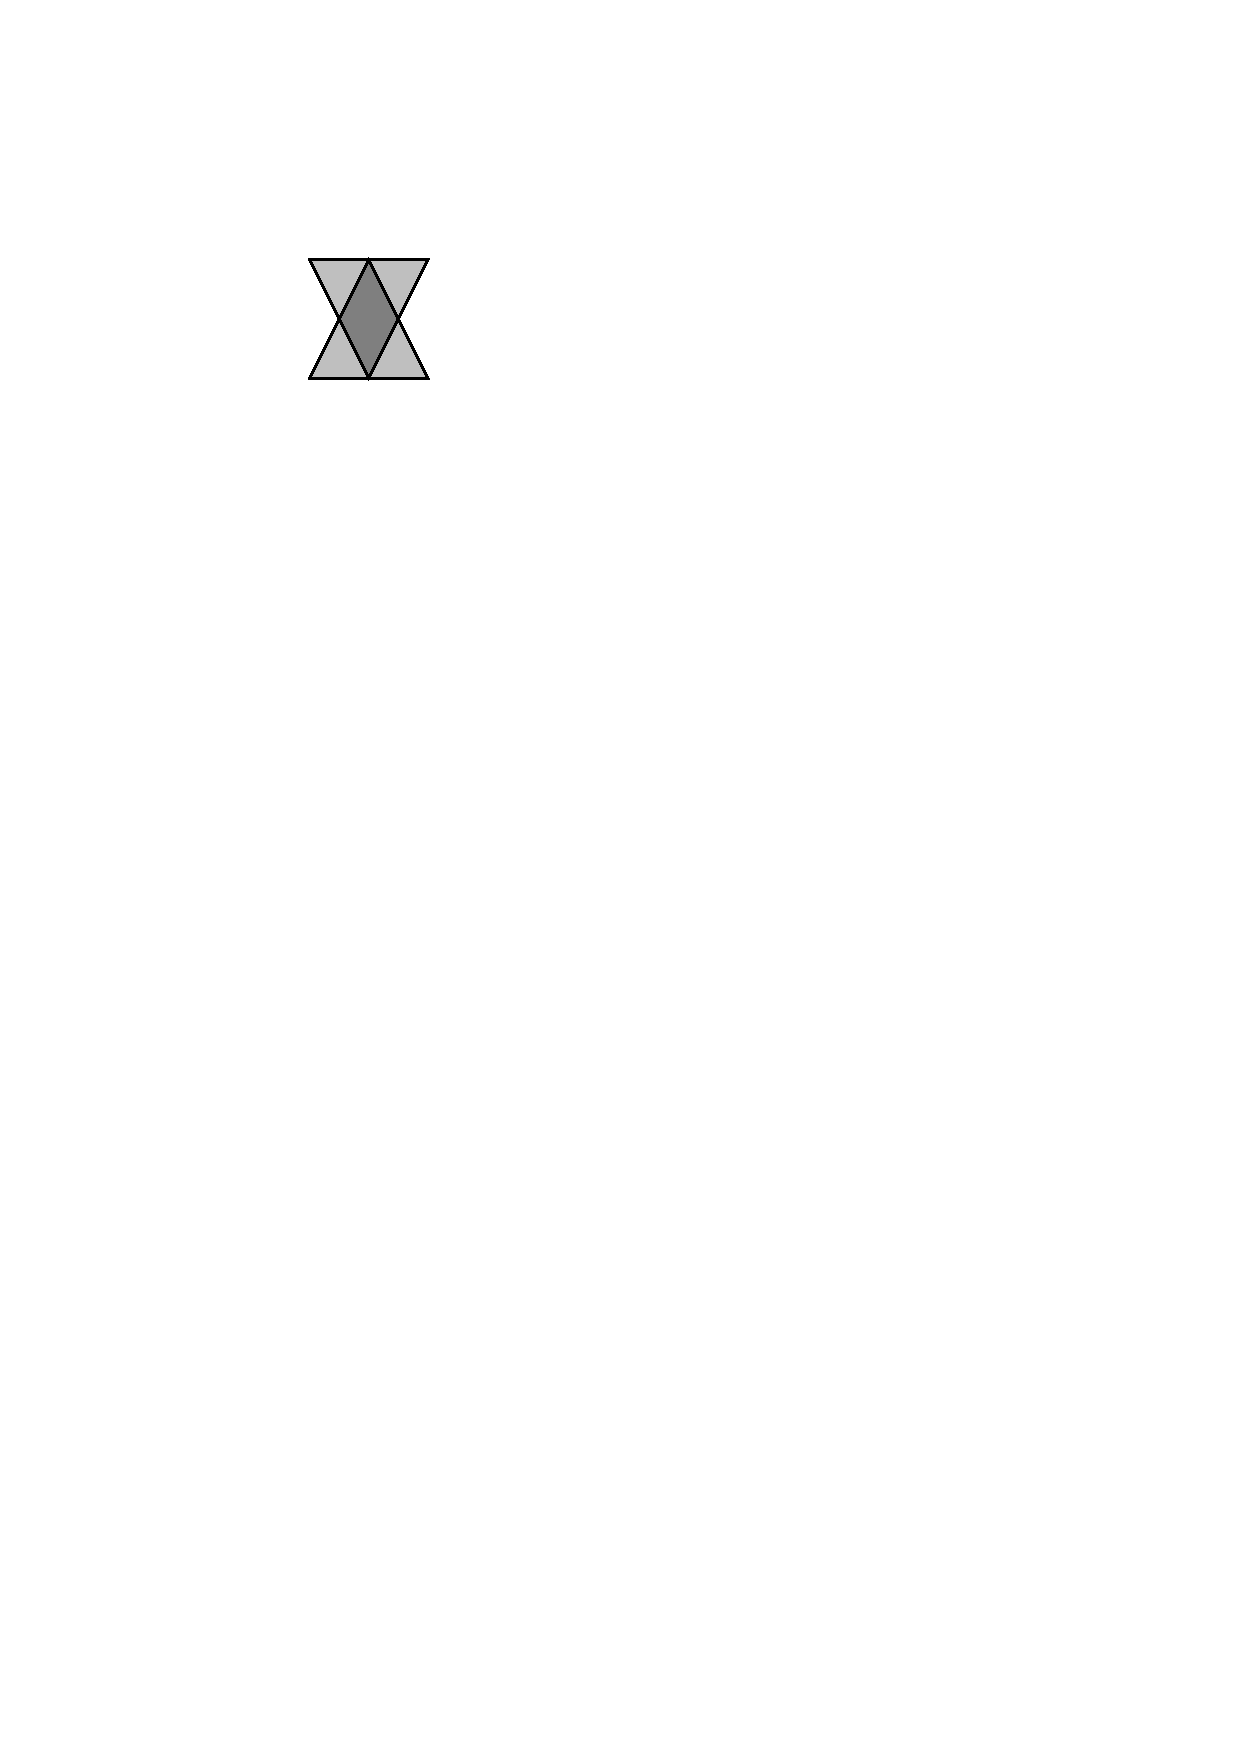
\includegraphics{Boolean_set_operations_2/fig/triangles}
    \end{center}
  \end{minipage}
}

\lcTex{\vspace{-20pt}}
\ccIncludeExampleCode{../examples/Boolean_set_operations_2/ex_do_intersect.C}

% ===============================================================
\section{General Polygons with Holes}
\label{bso_sec:general_polygons_with_holes}
% ===============================================================
Regular sets are closed under regularized Boolean set-operations.
These operations accept as input, and may result as output, general
polygons with holes, which model the concept 
\ccc{GeneralPolygonWithHoles_2}. This concept requires a type that
represents general polygons to be defined, namely \ccc{General_polygon_2}.
In addition, the concept requires access to the outer boundary, which is 
of type \ccc{General_polygon_2}, and to the holes, where each hole is also 
of type \ccc{General_polygon_2}. The outer boundary may be empty, in
which case the polygon is unbounded, and the number of holes may be zero. 
An unbounded polygon without holes spans the entire plane. Vertices of holes
and vertices of the boundary may coincide. The vertices of the outer
boundary are ordered counterclockwise, while the order the vertices
of each hole is clockwise.

The exact definition of the obtained general polygon with holes as a
result of a Boolean set-operation or a sequence of such operations is
closely related to the definition of regularized Boolean 
set-operations, being the closure of the interior of the corresponding
ordinary operation as explained next. There are many ways to arrive at a 
particular regular set. For example, the regular set depicted to the left 
is the result of the union of three small triangles translated 
appropriately. It is also the result of the difference between
\lcTex{%
  \setlength{\widthRight}{1.4cm}
  \setlength{\widthLeft}{\widthLineReal}
  \addtolength{\widthLeft}{-\widthRight}
  \begin{minipage}{\widthLeft}
}
\label{fig:unique}
\begin{ccHtmlOnly}
  <p><center>
    <img src="./fig/fig_unique.gif" border=0 alt="Unique" align=left>
  </center>
\end{ccHtmlOnly}
a large
triangle and a small upside down triangle. However the set of polygons
with holes obtained by the user through the application of any sequence
of operations is unique. 
The point set depicted to the left is represented 
as a single general polygon with holes that has a single hole 
(and not as three polygons with holes that have no holes at all). The
boundaries of the holes in a general polygon with holes are parts of the 
polygon (and not the holes), and as a general rule, if two point sets are
connected, then they belong to the same polygon with holes.
\lcTex{%
  \end{minipage}\hspace{\minipageSpace}
  \begin{minipage}{\widthRight}
    \begin{center}
    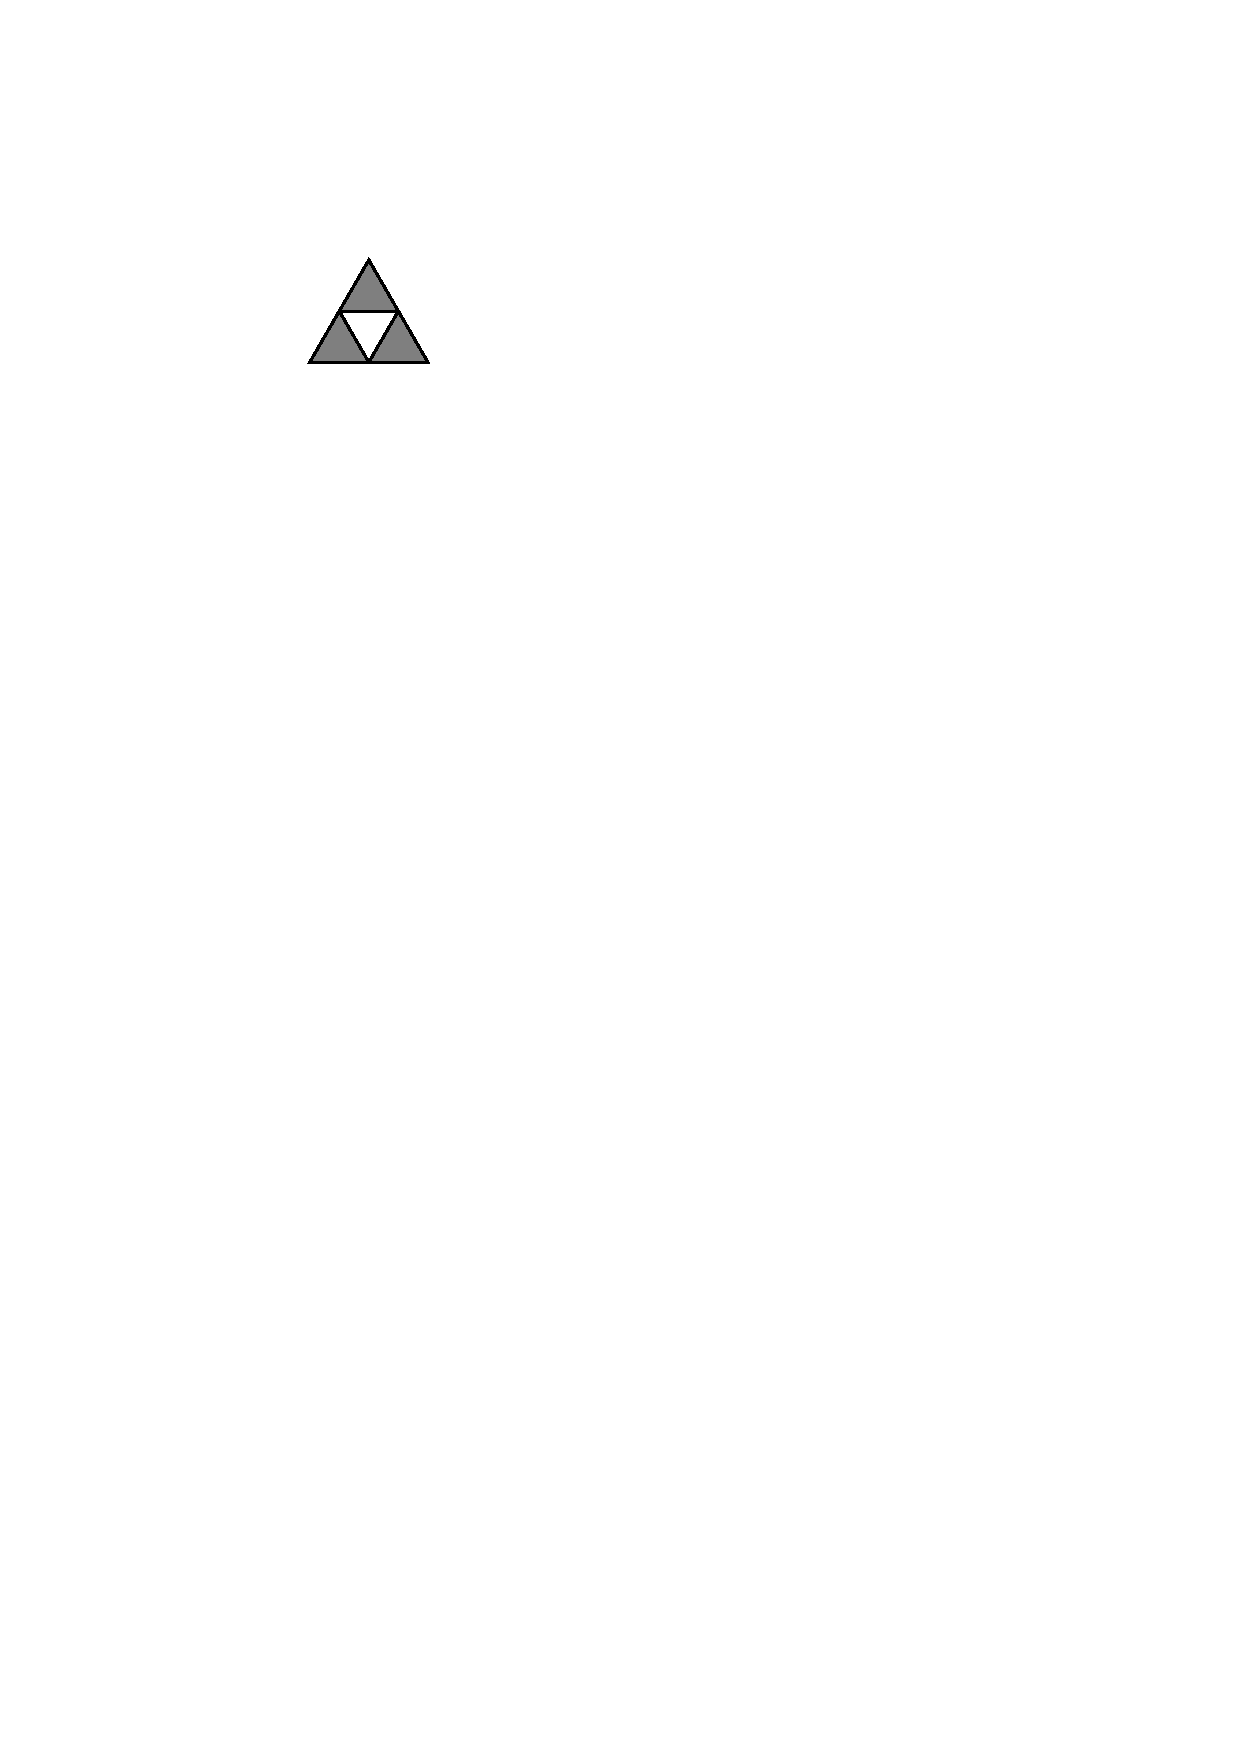
\includegraphics{Boolean_set_operations_2/fig/unique}
    \end{center}
%    Triangles.
  \end{minipage}
}
 
Instances of \ccc{General_polygon_2} used as input must be strictly simple
as a precondition. Instances of \ccc{General_polygon_2} obtained as output
are guaranteed to be strictly simple. On the other hand, neither the outer
boundary, nor any one of the holes, of an instance of
\ccc{General_polygon_with_holes_2} used as input, or obtained as output,
must be strictly simple.

% ---------------------------------------------------------------
\section{Free Functions}
\label{bso_sec:free_functions}
% ---------------------------------------------------------------
In many cases a simple operation that operates on two strictly simple
polygons that have no holes are required. The most simple functions in
the package operate on two polygons and accept them as two separate
parameters. However, even a simple operation, such as the union of two
strictly simple polygons with no holes, may result with a polygon with
holes, see Figure~\ref{fig:simple}~(a). Moreover, a simple operation,
such as the intersection of two strictly simple polygons with no holes, 
may result with a set of disjoint polygons; see
Figure~\ref{fig:simple}~(b). Finally, only a polygon with holes can
represent the complement of a polygon without holes. Notice that this
polygon has no outer boundary; see Figure~\ref{fig:simple}~(c).

\begin{figure}[!htp]
\begin{ccTexOnly}
\begin{center}
\begin{tabular}{ccc}
\pspicture[](0,0)(3,2)
\psset{unit=1cm,linewidth=1pt}
  \pspolygon*[linecolor=gray](0,1)(2,0)(1,1)(2,2)
  \pspolygon*[linecolor=gray](3,1)(1,2)(2,1)(1,0)
  \pspolygon(0,1)(2,0)(1,1)(2,2)
  \pspolygon(3,1)(1,2)(2,1)(1,0)
\endpspicture &
\pspicture[](0,0)(5,2)
\psset{unit=1cm,linewidth=1pt}
  \pspolygon*[linecolor=lightgray](0,0)(1.5,1.5)(2.5,0.5)(3.5,1.5)(5,0)
  \pspolygon*[linecolor=lightgray](0,2)(5,2)(3.5,0.5)(2.5,1.5)(1.5,0.5)
  \pspolygon*[linecolor=gray](1,1)(1.5,1.5)(2,1)(1.5,0.5)
  \pspolygon*[linecolor=gray](3,1)(3.5,1.5)(4,1)(3.5,0.5)
  \pspolygon(0,0)(1.5,1.5)(2.5,0.5)(3.5,1.5)(5,0)
  \pspolygon(0,2)(5,2)(3.5,0.5)(2.5,1.5)(1.5,0.5)
\endpspicture &
\pspicture[](0,0)(3,2)
\psset{unit=1cm,linewidth=1pt}
  \pspolygon*[linecolor=gray](0,2)(0,0)(3,0)(3,2)
  \pspolygon*[linecolor=lightgray](1,0.67)(2,0.67)(2,1.34)(1,1.34)
  \pspolygon[linecolor=black](1,0.67)(2,0.67)(2,1.34)(1,1.34)
\endpspicture
\\
(a) & (b) & (c)
\end{tabular}
\end{center}

\end{ccTexOnly}
\begin{ccHtmlOnly}
  <p><center>
    <img src="./fig/simple.gif" border=0 alt="Operations on Strictly
    simple polygons">
  </center>
\end{ccHtmlOnly}
\caption{\label{fig:simple}Operations on strictly simple polygons. (a) The union of two
strictly simple polygons. (b) The intersection of two strictly simple
polygons. (c) The complement of a strictly simple polygon.} 
\end{figure}

Many free functions that implement the regularized Boolean 
set-operations are parameterized by the two abstract types of the polygons 
used to represent the operands of the operation. If the result of an 
operation is not a Boolean value, as in the case of computing the 
intersection of two polygons, it is provided through a single polygon with 
holes or an output iterator of a range of polygons with holes. The example
below computes the intersection of two general polygons depicted in 
Figure~\ref{fig:simple}~(b), and inserts the resulting polygons into a 
container through an output iterator. Then, it computes the union of the
same input polygons and pushes the resulting polygon with holes at the
back of the same container. 

Suppose that you need to compute the union of two general polygons. If the
two polygons are disjoint, the result is a pair that consists of the two 
original polygons. Otherwise, it is a single general polygon perhaps with 
holes. This observation is used to simplify the interface of the free
functions that compute the union of two general polygons. These functions
return \ccc{false} iff the polygons are disjoint, and \ccc{true} otherwise,
in which case the resulting general polygon is placed in a third argument 
passed by reference.

\ccIncludeExampleCode{../examples/Boolean_set_operations_2/ex_intersection.C}

% ===============================================================
\section{The Main Component}
\label{bobs_sec:main_component}
% ===============================================================
The central component in the Boolean Set-Operations package is the
\ccc{General_polygon_set_2} class-template. It employs the
\ccc{Arrangement_2} class to represent a point set in the plane as a
planar arrangement; see Chapter~\ref{chapterArrangement_2}. 
Every point set that can be represented by an instance $R$ of the 
\ccc{General_polygon_set_2} type has a unique internal representation 
as a (unique) planar arrangement regardless of the particular sequence 
of operations that were applied to arrive at $R$. 
An instance of the \ccc{General_polygon_set_2} class-template can be
constructed from general polygons or general polygons with holes.
The class template provides methods to apply regularized Boolean 
set-operations on pairs of instances of \ccc{General_polygon_set_2} 
or general polygon (or general polygon with holes) directly, and a few
other utility methods, with the method to compute the complement being 
an exception, as it accepts a single instance of one of the types above. 
The input and output of these methods consist of one or more general 
polygons, some of which may have holes.

As mentioned above, the package also contains free functions that perform 
common operations, and are provided for convenience. A typical such function 
constructs a pair of \ccc{General_polygon_set_2} instances, invokes the 
appropriate method to apply the desired Boolean operation, and results with 
a Boolean value or at least one polygon. When several operations are 
performed in a sequence, it is much more efficient to use the member 
functions of the \ccc{General_polygon_set_2} type directly, as the 
extraction of the polygons from the internal representation for some 
operation, and the reconstruction of the internal representation for 
the succeeding operation could be time consuming.

% ---------------------------------------------------------------
\subsection{A Sequence of Boolean Set Operations}
\label{bso_ssec:sequence}
% ---------------------------------------------------------------
Member functions of the \ccc{General_polygon_set_2} that perform the
Boolean set-operations come in two flavours as follows. Some of the 
methods accept two arguments that represent two operands. These methods 
store the result in a third instance, the current object. Their 
counterpart methods accept only a single argument that represents one of 
the operands. The other one is provided by the current instance, which is 
replaced by the result. Similarly, one flavour of the \ccc{complement()} 
method accepts a single argument that represents the (single) operand, 
and the other one applies the operation on the current instance.

The next example performs a sequence of three Boolean set-operations.
First, it computes the union of two simple polygons depicted in
Figure~\ref{fig:simple}~(a). Then, it computes the complement of the result
of the union operation. Finally, it computes the intersection of the result
of the complement operation with a rectangle, confining the final result to 
the area of the rectangle.

\ccIncludeExampleCode{../examples/Boolean_set_operations_2/ex_sequence.C}

% ---------------------------------------------------------------
\subsection{Inserting non Intersecting Polygons}
\label{bso_ssec:insert}
% ---------------------------------------------------------------
If you want to compute the union of a polygon $P$ with a
general-polygon set $R$, and store the result in $R$, you can construct
a polygon set $S(P)$, and apply the {\em union} operation to
$R$ providing $S(P)$ as input:

\begin{alltt}
General_polygon_2 S(P);
R.join(S);
\end{alltt}

As a matter of fact, you can apply the union operation directly:

\begin{alltt}
R.join(P);
\end{alltt}

However, if you know that the polygon does not intersect any one of the
polygons represented by $R$, you can use the more efficient method
\ccc{insert()}:

\begin{alltt}
R.insert(P);
\end{alltt}

Both methods \ccc{insert()} and \ccc{join()}, like many others, are 
overloaded, as there exist methods that accept a range of polygons. 
In case of the \ccc{insert} method, all the general polygons in the 
input range and the general polygons represented by
$R$ must be pairwise disjoint in their interiors.

% ===============================================================
\section{The Traits}
\label{bso_sec:traits}
% ===============================================================
\lcTex{%
  \setlength{\widthRight}{1.4cm}
  \setlength{\widthLeft}{\widthLineReal}
  \addtolength{\widthLeft}{-\widthRight}
  \begin{minipage}{\widthLeft}
}
\label{fig:general_polygon}
\begin{ccHtmlOnly}
  <p><center>
    <img src="./fig/fig_general_polygon.gif" border=0 alt="A general polygon" align=right>
  <a name="fig:general_polygon"></a>
  </center>
\end{ccHtmlOnly}
An ordinary polygon is a closed point set bounded by a piecewise linear 
curve, such as the entities represented by \cgal 's \ccc{Polygon_2} type. 
However, the geometric mappings of the polygon edges in our context are not
necessarily linear. The operations provided by this package operate on point 
sets bounded by $x$-monotone segments of general curves (e.g., conic arcs and 
rational arcs). The point set depicted on the right is an example of a 
general polygon bounded by $x$-monotone circular arcs. The central class 
\ccc{General_polygon_set_2} that offers
\lcTex{%
  \end{minipage}\hspace{\minipageSpace}
  \begin{minipage}{\widthRight}
    \begin{center}
    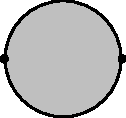
\includegraphics{Boolean_set_operations_2/fig/general_polygon}
    \end{center}
%    A general polygon.
  \end{minipage}
  \vspace{2pt}
}\\
methods that implement these operations is parameterized by a {\em traits}
class that defines the abstract interface between the operation and the 
geometric primitives used. The traits class models the traits concept 
\ccc{GeneralPolygonSetTraits_2}, and is tailored to handle a specific 
family of curves. The concept \ccc{GeneralPolygonSetTraits_2} refines the 
concept \ccc{ArrangementDirectionalXMonotoneTraits} specified next.

% ---------------------------------------------------------------
\subsection{The Traits Curves}
\label{bso_ssec:traits_curves}
% ---------------------------------------------------------------
The concept \ccc{ArrangementDirectionalXMonotoneTraits} refined the 
concept \ccc{ArrangementXMonotoneTraits_2}. Thus, a model of this 
concept must define the type \ccc{X_monotone_curve_2}, which represents 
an $x$-monotone curve, and the type of the curve endpoint \ccc{Point_2}, 
which represents a planar point. It also must provide various operations 
on these types listed by the base concept. This  concept requires two 
operations on $x$-monotone curves listed below in addition to those
required by base concept \ccc{ArrangementXMonotoneTraits_2}:
\begin{itemize}
\item Given an $x$-monotone curve, construct its opposite curve.
\item Given an $x$-monotone curve, compare its two endpoints 
lexicographically.
\end{itemize}
The main difference between the \ccc{ArrangementXMonotoneTraits_2}
and \ccc{ArrangementDirectionalXMonotoneTraits} concepts  is that a curve
of type \ccc{X_monotone_curve_2} type is considered to be directed by
the former. Namely, it has a source and a target points.

The traits classes \ccc{Arr_segment_traits_2}, 
\ccc{Arr_non_caching_segment_traits}, \ccc{Arr_rational_arc_traits_2},
and \ccc{Arr_conic_traits_2}, which are part of the \ccc{Arrangement_2} 
package distributed with \cgal, model the concept 
\ccc{ArrangementDirectionalXMonotoneTraits}, as they are extended with 
members functions that implement the two operations above.
The \ccc{Arr_polyline_traits_2} cannot be made a model of the, 
\ccc{ArrangementDirectionalXMonotoneTraits} concept, as the
$x$-monotone curve it defines is always directed from left to right. Thus, an
opposite curve cannot be constructed.

Just as with the case of computations using models of the 
\ccc{ArrangementXMonotoneTraits_2} concept, operations are robust only
when exact arithmetic is used. When inexact arithmetic is used,
(nearly) degenerate configurations may result in abnormal termination
of the program or even incorrect results.

% ---------------------------------------------------------------
\subsection{The Traits Polygons}
\label{bso_ssec:traits_polygons}
% ---------------------------------------------------------------
\lcTex{%
  \setlength{\widthRight}{1.4cm}
  \setlength{\widthLeft}{\widthLineReal}
  \addtolength{\widthLeft}{-\widthRight}
  \begin{minipage}{\widthLeft}
}
\label{fig:general_polygon_with_holes}
\begin{ccHtmlOnly}
  <p><center>
    <img src="./fig/general_polygon_with_holes.gif" border=0 alt="A general polygon with holes" align=right>
  </center>
\end{ccHtmlOnly}
Every model of the traits-class concept must also define the types
\ccc{Polygon_2} and \ccc{Polygon_with_holes_2}, and it must provide
sufficient operations on objects of these types to enable the Boolean 
set-operations.  The type \ccc{Polygon_2} represents a simple point-set 
in the plane, whose boundary curves are $x$-monotone. There are no 
requirements on this type besides being default and copy constructible and
assignable. In other words, the type \ccc{Polygon_2} does not necessari-
\lcTex{%
  \end{minipage}\hspace{\minipageSpace}
  \begin{minipage}{\widthRight}
    \begin{center}
    
\includegraphics{Boolean_set_operations_2/fig/general_polygon_with_holes}
    \end{center}
%    A general polygon with holes.
  \end{minipage}
  \vspace{1pt}
}\\
ly provide methods to access the curves of the polygon boundary, nor 
does it necessarily provide a constructor from a range of curves. Instead, 
the traits concept requires these operations. The type 
\ccc{Polygon_with_holes_2} corresponds to the concept 
\ccc{GeneralPolygonWithHoles_2}. Recall, that this concept 
requires access to the outer boundary, which is of type \ccc{Polygon_2}, 
and to the holes, where each hole is also of type \ccc{Polygon_2}.
% The \ccc{Triangle_2} and \ccc{Iso_rectangle_2} classes for example,
% which represent a triangle and a parallel-axis rectangle in
% $\mathrm{E}^2$ are special cases of convex general polygon. The a-priori
% knowledge of whether the input polygons are convex may sometimes expedite
% the operation or simplify the representation of the result. For example,
% the intersection of two convex polygons is either an empty polygon or a
% convex polygon.

% ---------------------------------------------------------------
\subsection{Types of Traits}
\label{bso_ssec:traits_types}
% ---------------------------------------------------------------
\lcTex{%
  \setlength{\widthRight}{2.4cm}
  \setlength{\widthLeft}{\widthLineReal}
  \addtolength{\widthLeft}{-\widthRight}
  \begin{minipage}{\widthLeft}
}
\label{fig:circle_recs}
\begin{ccHtmlOnly}
  <p><center>
    <img src="./fig/circles_rects.gif" border=0 alt="Union of circles
    and rectangles" align=right>
  </center>
\end{ccHtmlOnly}
Two traits classes are distributed with \cgal, namely 
\ccc{Gps_segment_traits_2} and \ccc{Gps_circle_segment_traits_2}. 
The former handles linear segments, and uses the \ccc{Polygon_2} type,
which is defined in the Polygons and Polygon Operations package of 
\cgal; see Chapter~\ref{Polygon}. The latter handles circular arcs
and linear segments concurrently. It is parameterized by a rational 
kernel, which makes it extremely efficient. The details are provided in the 
reference manual. The following example uses this traits class to compute
the union of four rectangles and four circles incrementally resulting with 
a single polygon with a single hole, as depicted on the right. Note that as
the four circles
\lcTex{%
  \end{minipage}\hspace{\minipageSpace}
  \begin{minipage}{\widthRight}
    \begin{center}
    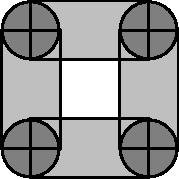
\includegraphics{Boolean_set_operations_2/fig/circles_rects}
    \end{center}
%    A general polygon with holes.
  \end{minipage}
  \vspace{2pt}
}\\
are disjoint, their union is computed with the \ccc{insert} method, 
while the union of the rectangles is computed with the \ccc{join} operator.

\ccIncludeExampleCode{../examples/Boolean_set_operations_2/ex_circle_segment.C}

% ===============================================================
\subsection{General Polygon Set Traits Adaptor}
\label{bso_ssec:general_polygon_concept}
% ===============================================================
The concept \ccc{GeneralPolygon_2} and its generic model 
\ccc{General_polygon_2<ArrDirectionalXMonotoneTraits>} facilitate the 
production of general-polygon set traits classes. A model of the concept 
\ccc{GeneralPolygon_2} represents a simple point-set in the plane bounded 
by $x$-monotone curves. As opposed to the plain \ccc{Traits::Polygon_2} type 
defined by any traits class, it must define the type 
\ccc{X_monotone_curve_2}, which represents an $x$-monotone curve of the 
point-set boundary. It must provide a constructor from a range of such 
curves, and a pair of methods, namely \ccc{curves_begin()} and 
\ccc{curves_end()}, that can be used to iterate over the point-set boundary 
curves.
 
The class-template \ccc{General_polygon_2<ArrDirectionalXMonotoneTraits>}
models the concept \ccc{GeneralPolygon_2}. Its template parameter must be
instantiated with a model of the concept
\ccc{ArrangementDirectionalXMonotoneTraits_2} from which it obtains the 
\ccc{X_monotone_curve_2} type, and it uses the necessary 
operations on this type provided by such a model to maintain a container 
of directed curves of type \ccc{X_monotone_curve_2}, which represents the 
boundary of the general polygon.

The class-template 
\ccc{Gps_traits_adaptor_2<ArrDirectionalXMonotoneTraits,GeneralPolygon>}
models the concept \ccc{GeneralPolygonSetTraits_2}. Its implementation is 
rather simple, as it is derived from the instantiated template-parameter 
\ccc{ArrXMonotoneTraits} inheriting its necessary types and methods, 
and it exploits the methods provided by the instantiated parameter 
\ccc{GeneralPolygon} --- a model of the concept \ccc{GeneralPolygon_2}.
By default, the \ccc{GeneralPolygon} parameter is defined as
\ccc{General_polygon_2<ArrangementDirectionalXMonotoneTraits_2>}

The code excerpt listed below defines a general-polygon set type that
can be used to perform Boolean set-operations on point sets bounded by
linear segments used by the \ccc{Arrangement_2} class by default. A
model of the \ccc{GeneralPolygon_2} concept that represents a
(linear) polygon bounded by curves of type \ccc{Arr_segment_2} is
generated. The later is obtained from the instantiated parameter
\ccc{Arr_segment_traits_2}, which defines \ccc{Arr_segment_2} to be
its exposed type \ccc{X_monotone_curve_2}.
\begin{alltt}
typedef CGAL::Gmpq                                             Number_type;
typedef CGAL::Cartesian<Number_type>                           Kernel;
typedef CGAL::Arr_segment_traits_2<Kernel>                     Arr_traits;
typedef CGAL::General_polygon_2<Arr_traits>                    General_polygon;
typedef CGAL::Gps_traits_adaptor_2<Arr_traits,General_polygon> Traits;
typedef CGAL::General_polygon_set_2<Traits>                    General_polygon_set;
\end{alltt}

\lcTex{%
  \setlength{\widthRight}{4.4cm}
  \setlength{\widthLeft}{\widthLineReal}
  \addtolength{\widthLeft}{-\widthRight}
  \begin{minipage}{\widthLeft}
}
\label{fig:conics}
\begin{ccHtmlOnly}
  <p><center>
    <img src="./fig/conic_arcs.gif" border=0 alt="Conic arcs" align=right>
  </center>
\end{ccHtmlOnly}
Swapping the linear arrangement-traits \ccc{Arr_segment_traits_2}
above with a traits class that handle conic arcs, such as
\ccc{Arr_conic_traits_2}, results with the definition of a
general-polygon set type that can be used to perform Boolean 
set-operations on point sets bounded by conic arcs of type
\ccc{Arr_conic_2}. The next example computes the intersection of the
two general polygons depicted in Figure~\ref{fig:conics}. One is an ellipse
given by $x^2 + 4y^2 - 4 = 0$, and the other is bounded by the two
parabolic arcs whose underlying parabola are given by 
$x^2 + y - 4 = 0$, and $x^2 - y - 4 = 0$. The code in the example adapts
the traits model that handles conics included with the \ccc{Arrangement_2}
package.
\lcTex{%
  \end{minipage}\hspace{\minipageSpace}
  \begin{minipage}{\widthRight}
    \begin{center}
    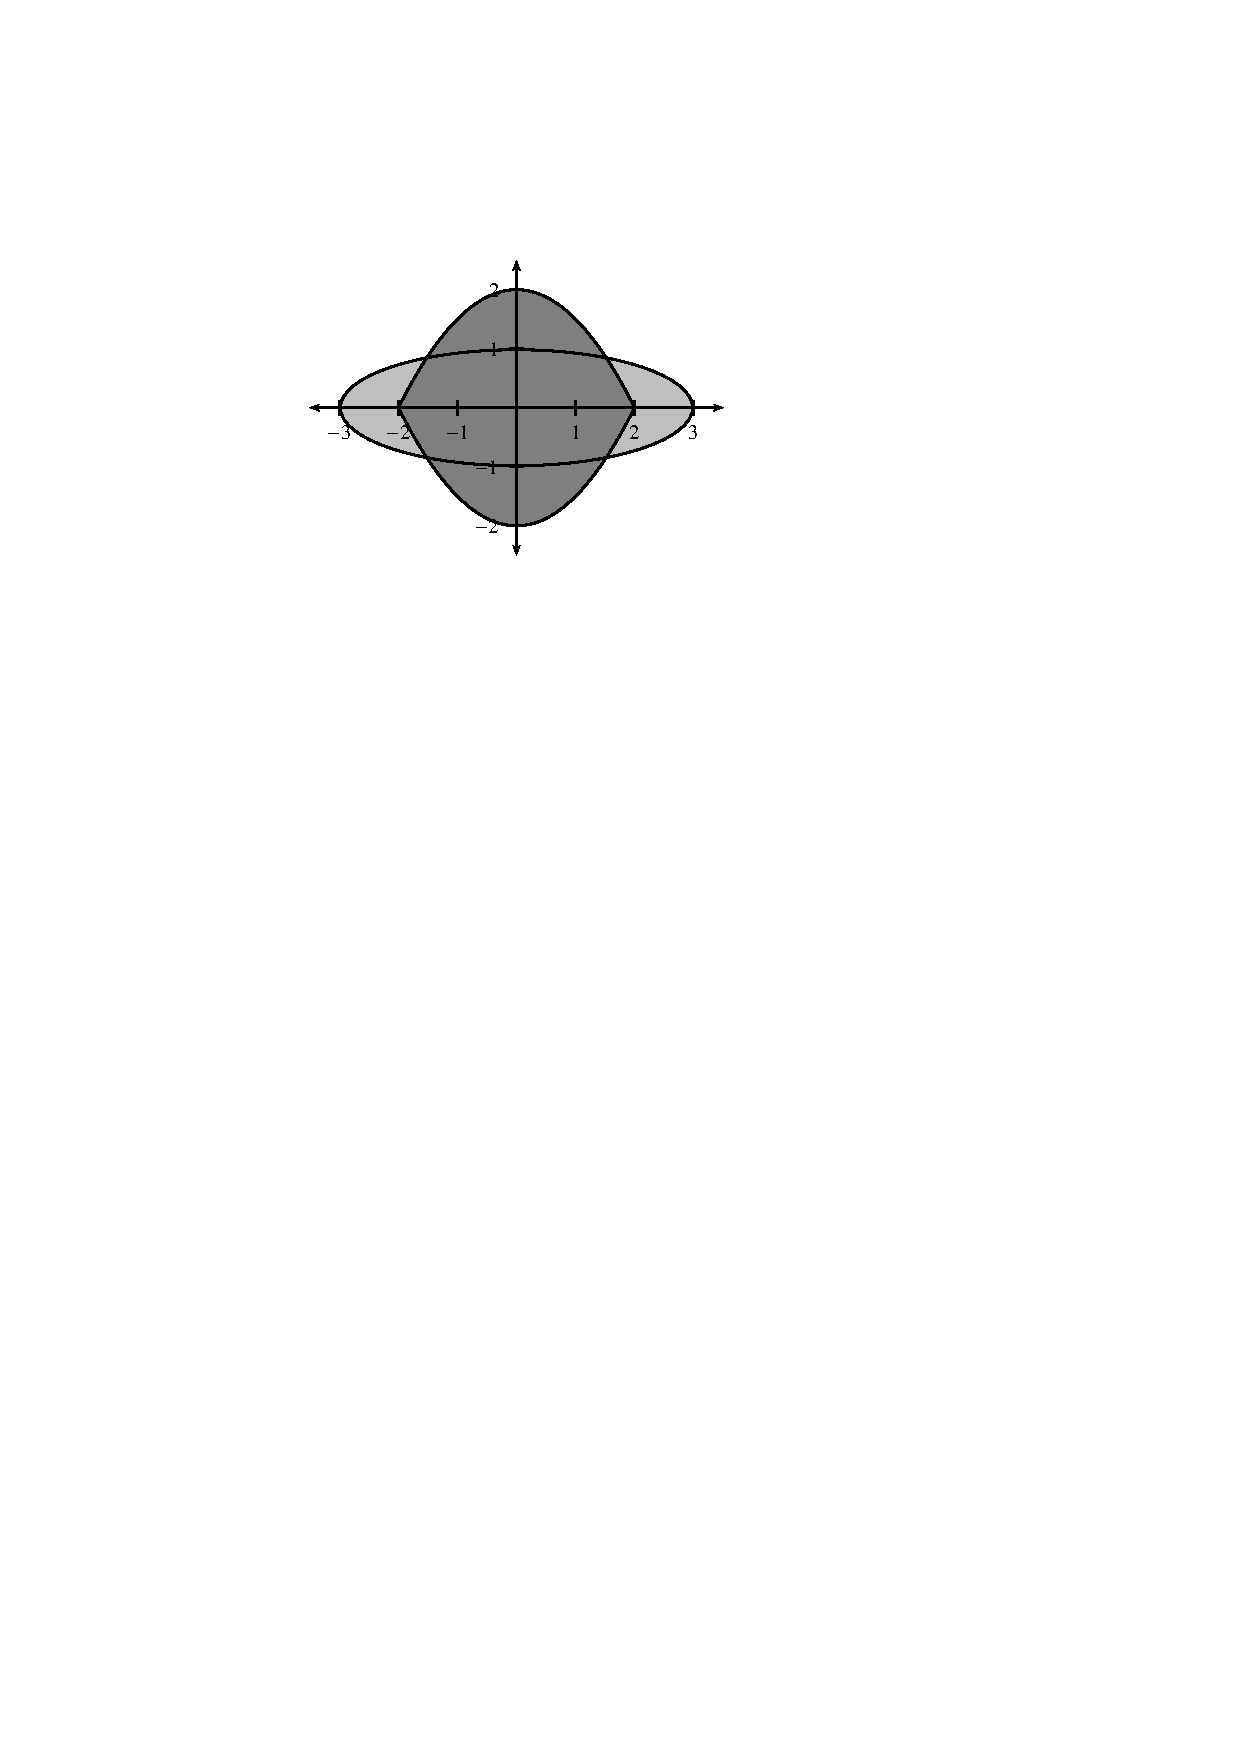
\includegraphics{Boolean_set_operations_2/fig/conic_arcs}
% Conic arcs.
    \end{center}
  \end{minipage}
}

\ccIncludeExampleCode{../examples/Boolean_set_operations_2/ex_traits_adaptor.C}

% ===============================================================
\subsection{Aggregated Operations}
\label{bso_ssec:}
% ===============================================================
\lcTex{%
  \setlength{\widthRight}{3.4cm}
  \setlength{\widthLeft}{\widthLineReal}
  \addtolength{\widthLeft}{-\widthRight}
  \begin{minipage}{\widthLeft}
}
\label{fig:disks}
\begin{ccHtmlOnly}
  <p><center>
    <img src="./fig/disks.gif" border=0 alt="Union of disks" align=right>
  </center>
\end{ccHtmlOnly}
If you wish to compute the union of a set of general polygons, you can
do it incrementally, computing the union of pairs of polygons one at a
time, until you arrive at the final solution. However, this operation
can be done much more efficiently, if all the polygons in the entire
set are operated at once. The package provides a free function that
aggregately computes the union of a set of polygons. There is no
restriction on the polygons in the set. Naturally, they may intersect
each other. Similarly, the package provides a free function that
determines whether a set of general polygons intersect, a function
that computes the intersection of a set of general polygons, and
functions that computes the difference and symmetric difference between 
the union of two sets of general
\lcTex{%
  \end{minipage}\hspace{\minipageSpace}
  \begin{minipage}{\widthRight}
    \begin{center}
    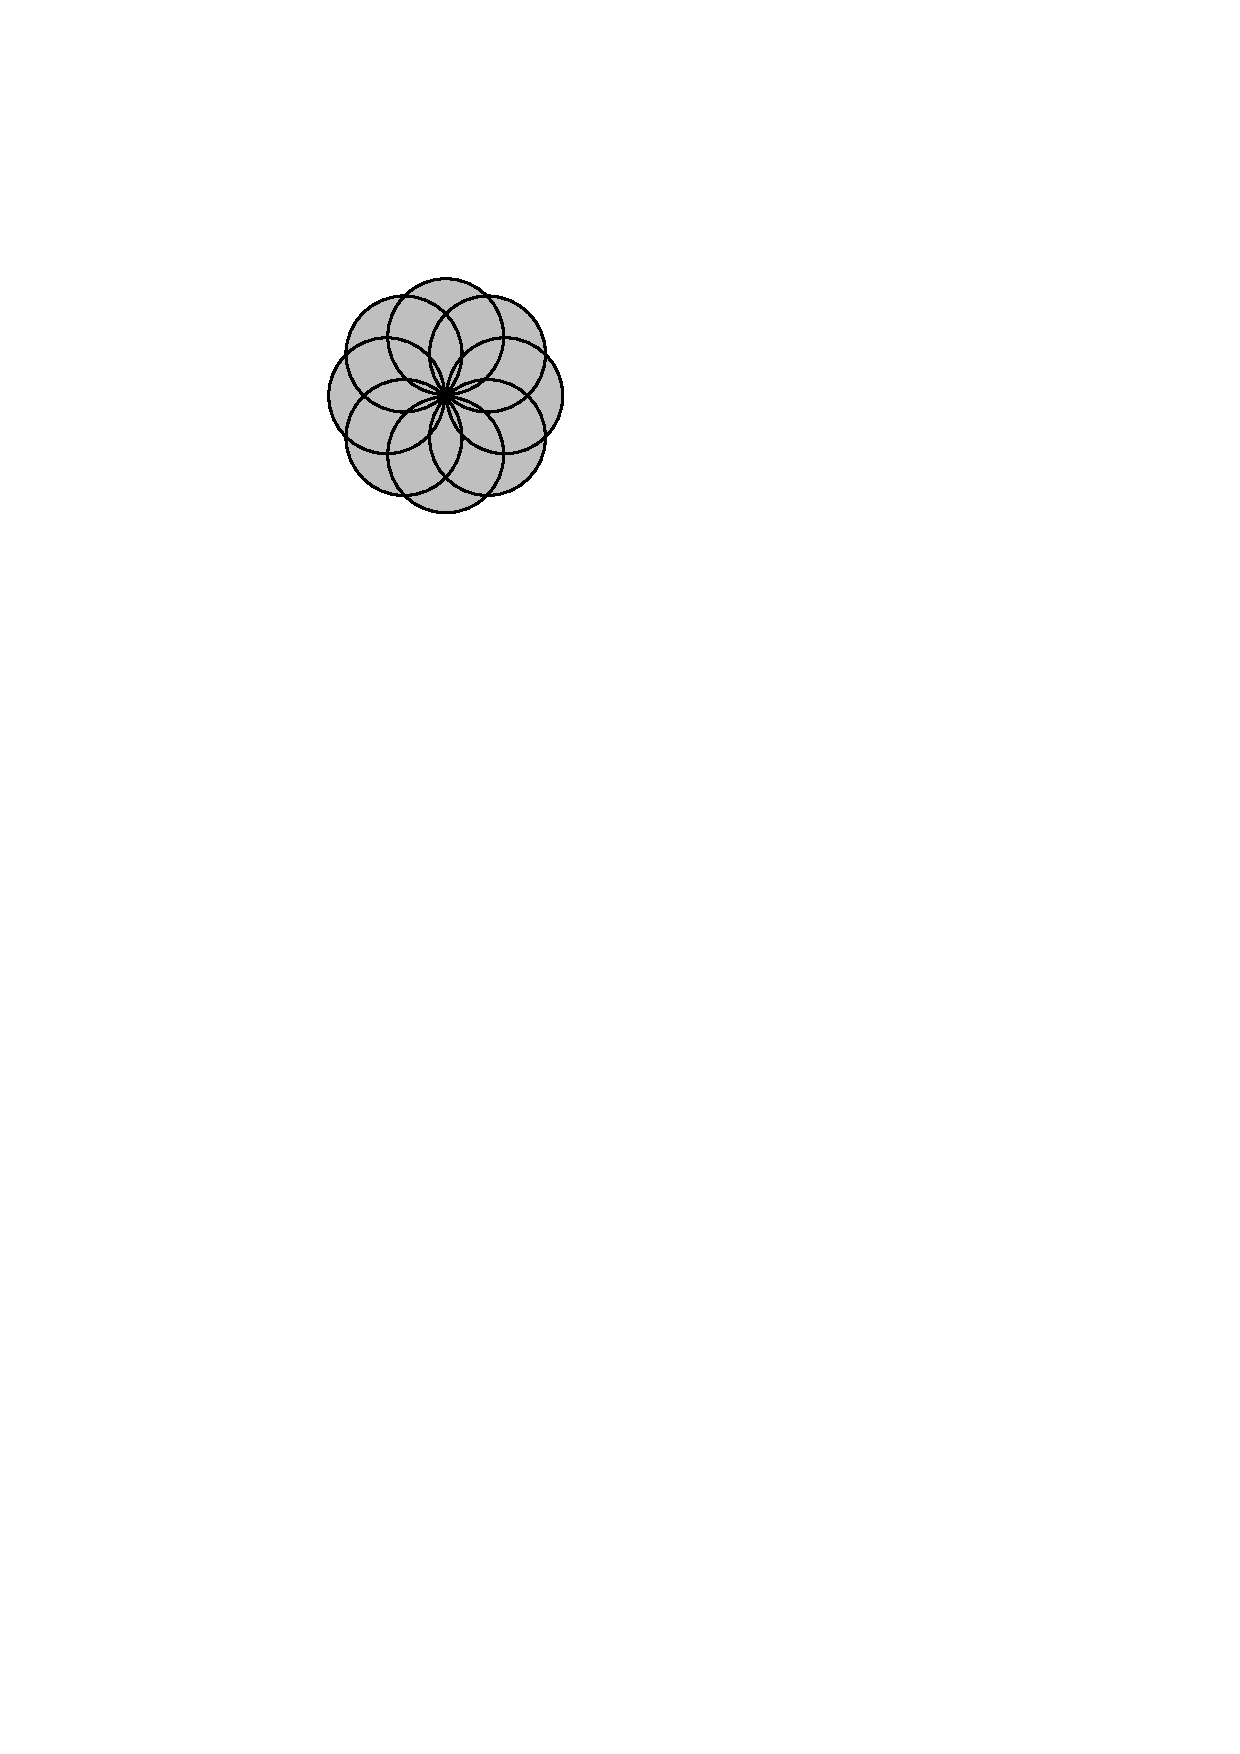
\includegraphics{Boolean_set_operations_2/fig/disks}
    \end{center}
%    Union of disks.
  \end{minipage}
\vspace{2pt}
}\\
polygons. The class \ccc{General_polygon_set_2} has the equivalent 
member functions. When such a member function is called, the general 
polygons represented by the current object are considered operands as 
well. In case of aggregately computing the difference or symmetric 
difference, the general polygons represented by the current object 
comprise the first set. The aggregated operations are based on the 
sweep-line paradigm. 

The next example computes the union of eight disks represented by
eight circles respectively depicted in Figure~\ref{fig:disks}. Each
circle is split into two $x$-monotone circular arcs that represent a
general polygon. The union operation is applied to the range of
general polygons spanning the list of the eight disks.

\ccIncludeExampleCode{../examples/Boolean_set_operations_2/ex_set_union.C}
